Un primo approccio di analisi è stato quello di cercare una corrispondenza, tramite ricerca per codici hash, tra i file presenti sulla memoria USB e l'HDD acquisito.\vspace{14pt}\\
Viene quindi creato un \textbf{Hash Set} all'interno di Autopsy per effettuare la ricerca su tutti gli \textbf{MD5} inerenti ai file presenti nella USB.
\begin{center}
    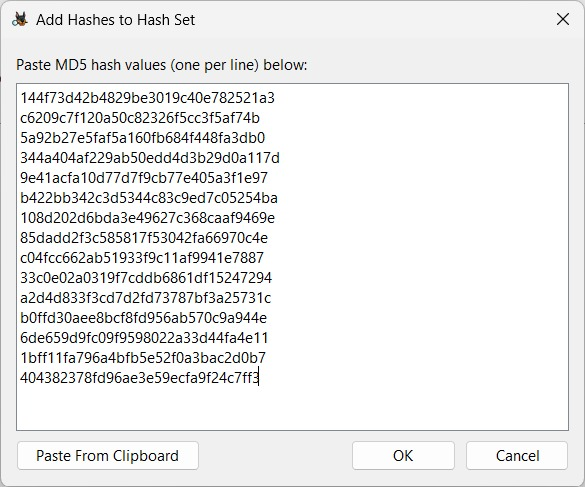
\includegraphics[width=0.7\textwidth]{img/hash-list.jpeg}
\end{center}
Una volta salvato l'Hash Set, Autopsy esegue la \textbf{ricerca tramite Hash} all'interno dell'HDD trovando \textbf{soltanto un unico Hashset Hit}.
\begin{center}
    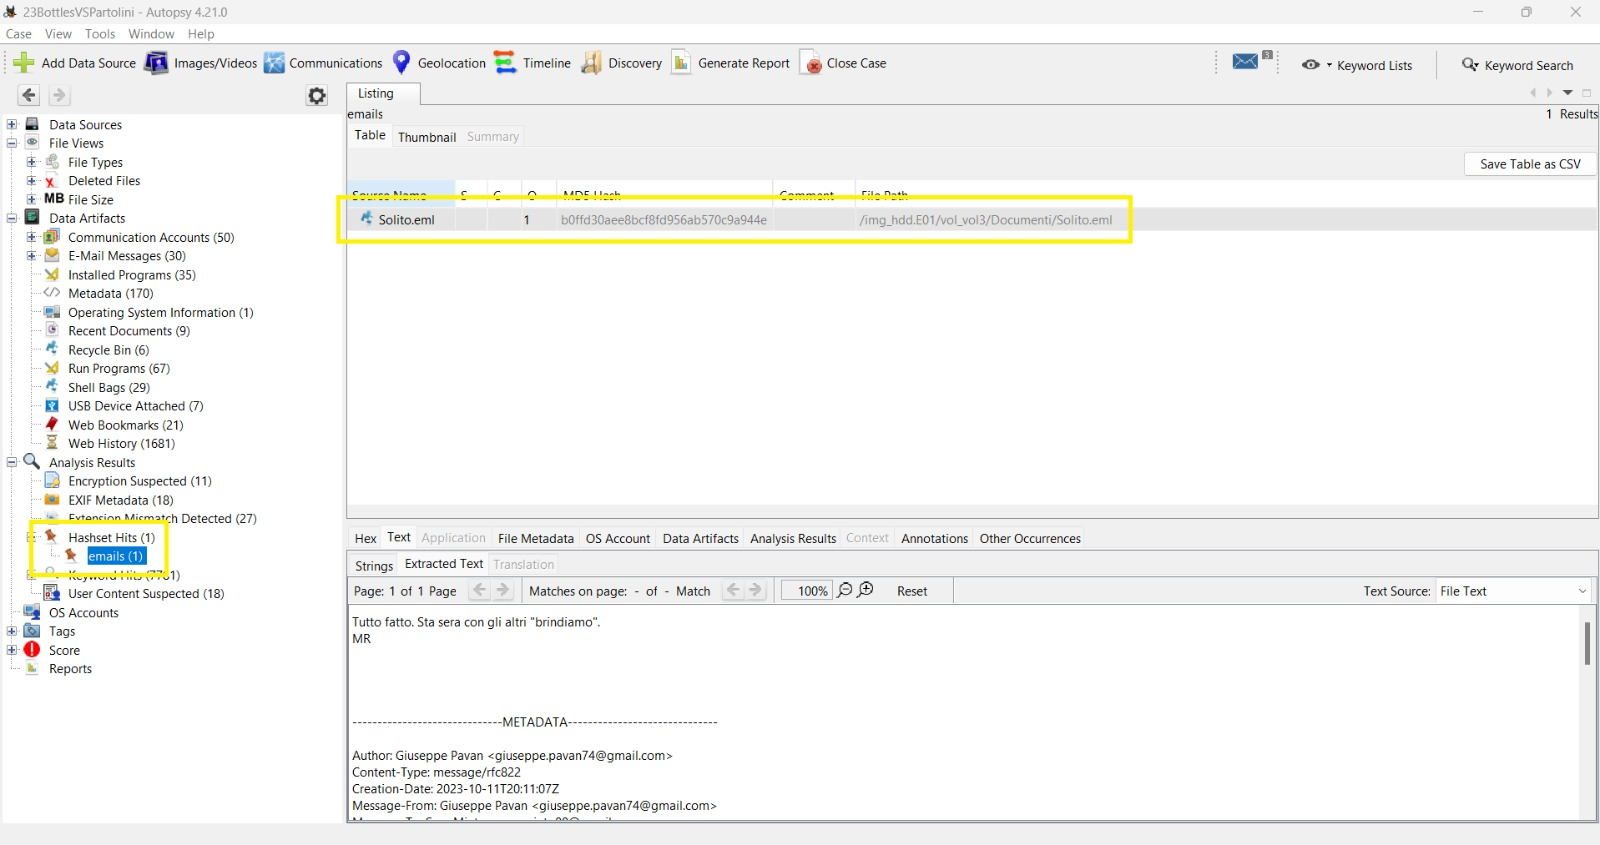
\includegraphics[width=1\textwidth]{img/hash-result.jpeg}
\end{center}
L'Hashset Hit riguarda l'unica email trovata all'interno dell'HDD sequestrato, ovvero la email "\textbf{Solito.eml}" [\ref{email10}].